\section{Arquitectura de la propuesta}

\section{Componentes}
Los componentes de la arquitectura se dividen en tres módulos principales. El primero corresponde al árbol de decisión, entrenado mediante la biblioteca scikit-learn de Python. El segundo está constituido por el código XDP, el cual incluye una parte autogenerada a partir del árbol de decisión. Finalmente, el tercer módulo es el entorno Mininet, empleado para la ejecución de pruebas en un entorno virtual local. Cabe destacar el fichero DecisionTree/arbolrw.py, encargado tanto del entrenamiento del árbol de decisión como de la autogeneración del código C, apoyándose para ello en una plantilla Jinja.

\subsection{Árbol de decisión}
El conjunto de datos empleado para el entrenamiento del árbol de decisión se ha generado a partir de un fichero CSV de 294,6 MB elaborado por el autor. Para su creación, se utilizó la versión más reciente del script pcap2csv.py, el cual permite la unión de dos o más ficheros PCAP en un único fichero CSV, así como la diferenciación entre paquetes de tráfico malicioso y legítimo mediante el uso de las banderas -l y -m. El script almacena únicamente información de los paquetes hasta el nivel de aplicación, sin analizar el contenido de este nivel, debido a la complejidad que supone obtener dichos datos en C a nivel de kernel.

El proceso de conversión comienza definiendo un diccionario con todas las posibles características que puede tener un paquete de red. A continuación, se leen los paquetes uno a uno y cada uno se procesa mediante una función que devuelve un diccionario en el que cada clave corresponde al nombre de una columna y cada valor al dato asociado a ese paquete en particular (véase un fragmento de esta función en \ref{pcap2dict}). En caso de que un paquete carezca de alguno de los campos —por ejemplo, los relativos a IP—, dichos valores se registran como None en lugar de omitirse, con el fin de mantener un formato uniforme en el CSV y evitar errores durante el procesamiento posterior.

Una vez transformado el paquete en diccionario, se añade al final la etiqueta ``Yes'' si corresponde a una muestra de ransomware, o ``No'' en caso contrario. Posteriormente, el diccionario se incorpora a un array. Cuando dicho array alcanza los 1024 elementos, su contenido se vuelca al fichero CSV y se vacía para liberar memoria. Este procedimiento se repite hasta procesar todos los paquetes, momento en el que se realiza un último volcado con los datos restantes. Se ha optado por este método de lectura y escritura para optimizar tanto el uso de memoria como la frecuencia de accesos de escritura al disco.

Los ficheros PCAP correspondientes al tráfico de ransomware fueron obtenidos, tal y como se explica en el apartado 2.1 por el trabajo de Eduardo Berrueta et al. entre los años 2015 y 2022\cite{qnyn-q136-20}. Por otro lado, el fichero PCAP con tráfico legítimo fue generado por el autor mediante la captura de tráfico durante una jornada laboral en un laboratorio universitario, registrando el uso normal de los dispositivos y recogiendo tráfico de protocolos como HTTP, HTTPS, DNS, SSH, entre otros. Con el objetivo de incrementar la precisión del árbol de decisión, se generó adicionalmente tráfico SMB2 mediante la copia de un fichero de gran tamaño a una unidad de almacenamiento ubicada en el CPD de la universidad.

En el proceso de preparación del dataset, se eliminaron las direcciones IP, las direcciones MAC y el timestamp de los paquetes, debido al número limitado presente tanto en las capturas de tráfico malicioso como en las de tráfico legítimo. Con ello, se evitó que el árbol de decisión se apoyara en características poco representativas o irrelevantes para un entorno real. Como métrica de calidad se mantuvo el índice de Gini, dada su fiabilidad y buen rendimiento, y como estrategia de división se empleó el criterio best. Aunque se preveía que el aumento del tamaño del dataset respecto a las pruebas podría incrementar el tiempo de entrenamiento, en la práctica no se observó un impacto significativo. En caso contrario, se habría considerado cambiar la estrategia a random. En cuanto a la profundidad máxima del árbol, se fijó inicialmente en cuatro niveles, ya que en pruebas previas con otros datasets de paquetes de red no se apreciaron mejoras de precisión al superar este valor.

Para entrenar el árbol de decisión, una vez definidas las columnas que serán eliminadas, se establece la variable x como el conjunto de columnas que forman parte de los datos de entrada y la variable y como la columna correspondiente al clasificador. A continuación, mediante la función \verb|train_test_split|, se divide el conjunto de datos de forma aleatoria, asignando el 80\% de las filas al entrenamiento y el 20\% restante a las pruebas, con el fin de evaluar la fiabilidad del modelo. Una vez realizada esta partición, se procede a entrenar el árbol utilizando los parámetros seleccionados y los datos de entrenamiento. Finalmente, se puede calcular la exactitud del modelo, si bien es recomendable interpretar este valor con cautela, dado que no siempre refleja de forma completamente sólida la capacidad de generalización del clasificador. El código correspondiente al entrenamiento del árbol puede consultarse en \ref{entrenamientoArbol}

Durante el desarrollo, se detectó que, por error, se había incluido la variable \verb|eth_type| en la lista de columnas excluidas del entrenamiento. Tras corregir esta omisión y volver a entrenar el modelo, se observó que la precisión se mantenía, pero esta vez con un nivel menos de profundidad, alcanzando una profundidad máxima de tres niveles a pesar de que el límite establecido era de cuatro. Este resultado sugiere que la inclusión de dicha variable aporta capacidad predictiva al modelo, optimizando su estructura sin pérdida de precisión.

\PythonCode[pcap2dict]{PCAP a Dict}{Fragmento de códgio que transforma parte de los datos de un paquete en un diccionario fácilmente convertible a CSV.}{../DecisionTree/pcap2csv.py}{39}{60}{39}

\PythonCode[entrenamientoArbol]{Entrenamiento Árbol}{Fragmento de códgio de arbolrw.py encargado de entrenar el árbol de decisión.}{../DecisionTree/arbolrw.py}{82}{111}{82}

\subsection{Código XDP y Código autogenerado}
Tal y como se indicó en el apartado 2.2, los programas XDP constan de dos componentes diferenciados. El primero de ellos es un programa escrito en C que se compila de forma convencional y cuya ejecución tiene lugar íntegramente en el espacio de usuario. El segundo componente corresponde a un programa que se traduce a bytecode y que, posteriormente, es cargado por el primero en el espacio del kernel, donde finalmente se ejecuta.

El programa de usuario inicia comprobando que se haya especificado la interfaz de red sobre la que se ejecutará el programa XDP y verificando que dicha interfaz exista efectivamente en el equipo. A continuación, mediante la función \verb|bpf_object__open_file|, el programa analiza el objeto XDP y prepara las estructuras necesarias en el espacio de usuario, como los mapas. Asimismo, se crea en memoria un \verb|struct bpf_object|, desde el cual se podrá acceder a estas estructuras en el espacio de usuario. Una vez preparado el entorno de usuario, se carga el bytecode correspondiente en el espacio de kernel mediante la función \verb|bpf_object__load|.

El programa C aún requiere el descriptor de archivo (file descriptor, FD) del mapa para poder interactuar con él, el cual se obtiene a través de la función \verb|bpf_object__find_map_fd_by_name|, que recibe como parámetros la estructura previamente creada y el nombre del mapa definido en el programa XDP. Por seguridad y persistencia, se fija el mapa en \verb|/sys/fs/bpf/| mediante la función \verb|bpf_obj_pin|; esto permite acceder al mapa incluso si el proceso que lo creó finaliza de forma inesperada y, además, sirve para comprobar si el mapa ya existe, lo que indica que el programa se ha ejecutado previamente o se encuentra en ejecución en ese momento. Como última tarea para terminar de cargar el programa XDP se obtiene el descriptor de archivo de la función principal del programa XDP a través de la función \verb|bpf_program__fd|, tras esto se adjunta dicha función al hook XDP que es el controlador de la gráfica a través de la función \verb|bpf_set_link_xdp_fd|. Una vez cargado el programa XDP, el programa de usuario se dedica a monitorizar los cambios del mapa y a mostrarlos en pantalla, dicho mapa contiene tanto el número de paquetes descartados como el número de paquetes que el programa XDP ha permitido pasar. En el fragmento de código \ref{xdp_usr} se muestra la sección del fichero XDP/arbol1/xdp\_usr.c que implementa las funciones principales previamente descritas.

\CCode[xdp_usr]{XDP Espacio de Usuario}{Fragmento de códgio que muestra como se carga el objeto, obtiene y fija el mapa y como se adjunta el programa al hook XDP}{../XDP/arbol1/xdp_usr.c}{28}{60}{28}

Se añadió la capacidad de autogenerar el código BPF/XDP una vez entrenado el árbol de decisión. Para ello, se recorre de forma recursiva el árbol y, en cada nodo, se genera la condición correspondiente a partir del nombre de la característica (previamente convertido a su nombre real) y del valor de umbral. Esta condición se pasa por una función que, en determinados casos, la sustituye por una equivalente válida. Por ejemplo, la condición \verb|src_port <= inf| se reemplaza por \verb#ip_proto == IPPROTO_TCP || ip_proto == IPPROTO_UDP#, dado que el hecho de que el puerto de destino sea menor que infinito únicamente implica que el puerto existe.

Cuando la condición resultante es válida, si corresponde al hijo izquierdo del nodo se inserta en una estructura if, mientras que si corresponde al hijo derecho se inserta en una estructura else. Para la generación del código se empleó una plantilla Jinja con la estructura prediseñada en C. Durante las pruebas, se observó que el mejor resultado se obtenía extrayendo los datos de las cabeceras IP antes de la evaluación del árbol, de forma que ya estuvieran disponibles en la plantilla. En caso de que el paquete analizado carezca de cabecera IP, dichos valores se establecen en cero.

\subsection{Mininet}
Mininet es un emulador de red que permite diseñar topologías compuestas por hosts finales, switches, routers (aunque de manera no nativa, ofreciendo únicamente el reenvío de paquetes) y enlaces dentro de un único kernel Linux. Además, dispone de una API accesible desde Python, lo que facilita el uso de este lenguaje de programación para la creación y configuración de las topologías de red\cite{lantz2021mininet}.

Como entorno de pruebas, se utilizó Mininet para implementar una topología inicial, que se muestra en la figura \ref{red-mininet-1}. Esta configuración consistía en dos hosts, cada uno conectado a un switch distinto, mientras que ambos switches se encontraban interconectados a un único router. Esta topología permitió realizar pruebas preliminares sobre el impacto del filtro basado en árboles de decisión en el rendimiento de la red.

Si bien esta configuración resultó útil para evaluar el funcionamiento básico del filtro, no era completamente representativa de un escenario real con una tarjeta de red equipada con DPU. Aunque dentro de la tarjeta los paquetes llegan al procesador de la DPU a través de Ethernet, la topología de Mininet no reproduce de manera exacta la interacción de los paquetes con el hardware especializado de la NIC. Al añadir más de una interfaz switch además del router, se introducen latencias adicionales que no existen en la NIC, por lo que este diseño inicial sirve únicamente para pruebas preliminares y no refleja completamente las condiciones de un entorno con DPU.

\begin{figure}[Primera Topología de Red]{red-mininet-1}{Primer diseño de topología de red usada en Mininet preliminares.}
	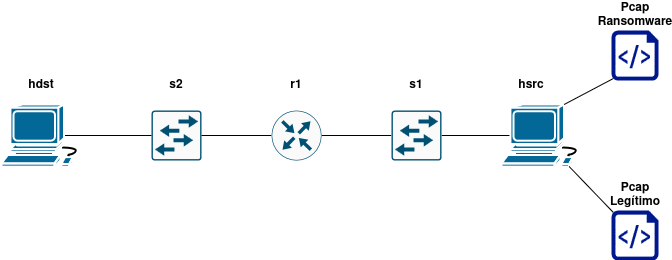
\includegraphics[width=0.9\textwidth]{capturas/DiagramaRedArbol1.png}
\end{figure}

Teniendo en cuenta que el entorno de pruebas real consiste en una tarjeta de red con dos puertos a nivel de enlace, se decidió simplificar la topología de Mininet para realizar pruebas más realistas. La red utilizada consta únicamente de dos host conectados a un único switch, eliminando la necesidad de routers adicionales o interfaces suplementarias tal y como se puede ver en la figura \ref{red-mininet-2}. Esta simplificación permite reducir la complejidad de la topología y minimizar factores externos que podrían afectar a las mediciones, como las latencias introducidas por componentes adicionales de la red virtual.

Además, esta configuración simplificada contribuye a disminuir la pérdida de paquetes durante las pruebas y reduce problemas relacionados con la resolución de direcciones MAC mediante ARP. Al aproximarse más al comportamiento de un entorno real con DPU, la topología proporciona un marco adecuado para medir el rendimiento de la red bajo la influencia del filtro de árbol de decisión. El siguiente paso en el proceso consistirá en realizar pruebas de rendimiento utilizando la herramienta iperf, lo que permitirá cuantificar de manera más precisa el impacto del filtrado sobre el tráfico de red.

\begin{figure}[Topología de Red Final]{red-mininet-2}{Diseño de topología de red usada en Mininet para pruebas.}
	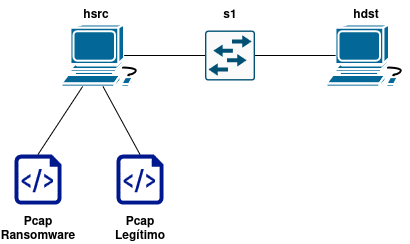
\includegraphics[width=0.55\textwidth]{capturas/DiagramaRed2.png}
\end{figure}

En los fragmentos de código \ref{redarbolrw} y \ref{redarbolrw1} se muestran extractos de los ficheros redarbolrw.py y redarbolrw1.py, correspondientes a la definición de la topología preliminar y de la topología definitiva, respectivamente.

\PythonCode[redarbolrw]{Red Árbol Preeliminar}{Fragmento de códgio que define la topología de red usada en las pruebas preeliminares.}{../Mininet/redarbolrw.py}{22}{54}{22}

\PythonCode[redarbolrw1]{Red Árbol Final}{Fragmento de códgio que define la topología de red usada en las pruebas finales.}{../Mininet/redarbolrw1.py}{8}{25}{8}
